% TrustLex -- IEEE conference paper (IEEEtran, two-column).
% Compile on Overleaf (pdfLaTeX) or locally with: latexmk -pdf trustlex.tex
\documentclass[conference]{IEEEtran}
\IEEEoverridecommandlockouts

\usepackage[T1]{fontenc}
\usepackage{cite}
\usepackage{amsmath,amssymb,amsfonts}
\usepackage{graphicx}
\usepackage{booktabs}
\usepackage{multirow}
\usepackage{array}
\usepackage{xcolor}
\usepackage{listings}
\usepackage{url}
\usepackage{tikz}
\usetikzlibrary{positioning,arrows.meta,fit}

\newcommand{\TL}{\textsc{TrustLex}}
\newcommand{\code}[1]{\texttt{#1}}
\newcommand{\lab}[1]{\textsf{\small #1}}

\newtheorem{theorem}{Theorem}

% Start a new row of author blocks (two authors per row).
\makeatletter
\newcommand{\linebreakand}{%
  \end{@IEEEauthorhalign}
  \hfill\mbox{}\par
  \mbox{}\hfill\begin{@IEEEauthorhalign}
}
\makeatother

\lstdefinelanguage{trustlex}{
  morekeywords={var,input,from,system,instruction,insert,sanitize},
  morecomment=[l]{\#},
  morestring=[b]",
}
\lstset{
  language=trustlex,
  basicstyle=\ttfamily\footnotesize,
  keywordstyle=\bfseries,
  commentstyle=\itshape\color{gray},
  stringstyle=\color{teal!70!black},
  columns=fullflexible,
  keepspaces=true,
  frame=single,
  framesep=2pt,
  xleftmargin=3pt,
  xrightmargin=3pt,
  aboveskip=4pt,
  belowskip=4pt,
}

\begin{document}

\title{TrustLex: Compile-Time Trust Typing for Injection-Safe Prompts in LLM-Integrated Applications}

\author{
\IEEEauthorblockN{Amritha Varshini Pakanati}
\IEEEauthorblockA{\textit{School of Computer Science}\\
\textit{and Engineering (SCOPE)}\\
\textit{Vellore Institute of Technology}\\
Vellore, Tamil Nadu 632014, India\\
amritha.varshini2024@vitstudent.ac.in}
\and
\IEEEauthorblockN{V L Lakshmi Shriyaa}
\IEEEauthorblockA{\textit{School of Computer Science}\\
\textit{and Engineering (SCOPE)}\\
\textit{Vellore Institute of Technology}\\
Vellore, Tamil Nadu 632014, India\\
lakshmishriyaa.vl2024@vitstudent.ac.in}
\linebreakand
\IEEEauthorblockN{Karthick Ganesh}
\IEEEauthorblockA{\textit{School of Computer Science}\\
\textit{and Engineering (SCOPE)}\\
\textit{Vellore Institute of Technology}\\
Vellore, Tamil Nadu 632014, India\\
karthick.ganesh2024@vitstudent.ac.in}
\and
\IEEEauthorblockN{Dr. Krishnaraj N}
\IEEEauthorblockA{\textit{School of Computer Science}\\
\textit{and Engineering (SCOPE)}\\
\textit{Vellore Institute of Technology}\\
Vellore, Tamil Nadu 632014, India\\
krishnaraj.n@vit.ac.in}
}

\maketitle

\begin{abstract}
Companies increasingly deploy large language models (LLMs) inside their own applications: support bots on websites, retrieval-augmented assistants over internal documents, and agents that consume tool and API results. Each application builds its prompt by concatenating the developer's trusted system prompt with untrusted text, so attacker-controlled text can impersonate the developer (prompt injection). We present \TL{}, a domain-specific language and compiler that makes trust a grammar-level type. Inputs declare their origin; the compiler tracks trust through variables, interpolation, concatenation and reassignment by exact symbolic evaluation over a five-level lattice, and refuses to compile any prompt in which untrusted data can reach the privileged system channel without a sanitizer, unless the input carries a refinement type that provably cannot express an instruction. We prove non-interference up to sanitization and validation and show that the check is complete for the language. Accepted programs compile to a checksummed, optionally HMAC-sealed intermediate representation that is bound at run time into OpenAI or Anthropic API payloads. On a labelled corpus \TL{} reaches an F1 score of 1.00 versus 0.55 for a lexical linter and 0.80 for a keyword filter; across 1{,}536 program--attack pairs it reduces structural leakage into the system prompt from 38.1\% to 0\%. In live experiments with three hosted models, using our own attacks and the public Tensor Trust benchmark, typed inputs block 100\% of attacks before any API call, and \TL{}'s layout significantly lowers indirect-injection success relative to placing the document in the user turn (e.g.\ from 73.0\% to 56.2\% on allam-2-7b with Tensor Trust attacks, $p=0.013$). Compilation takes about 5\,ms per program. The implementation, evaluation harness and results are available at \url{https://github.com/Karthick-Ganesh/TrustLex}.
\end{abstract}

\begin{IEEEkeywords}
prompt injection, large language models, information-flow control, security type systems, domain-specific languages, compilers, non-interference
\end{IEEEkeywords}

% =====================================================================
\section{Introduction}

Most real-world use of LLMs is not a person chatting with a model but an \emph{LLM-integrated application}: a company calls a general-purpose model through an API and wraps it in its own logic---a customer-support bot, a retrieval-augmented generation (RAG) assistant, an email assistant, or an agent that calls tools and web APIs. The model is not custom; the \emph{application} is. What makes it specific is its \emph{system prompt}---persona, business rules, restrictions---combined at run time with outside text.

The application builds its prompt by concatenating strings: developer instructions, the customer's message, a retrieved document, a tool result. The model receives one token sequence and cannot reliably tell who wrote which part. An attacker who controls any outside text can therefore write text that \emph{looks like} developer instructions: \emph{direct} injection through the customer message~\cite{perez2022ignore}, or \emph{indirect} injection planted in a document, web page or API response that the application later retrieves~\cite{greshake2023indirect}. OWASP ranks prompt injection as the top risk for LLM applications~\cite{owasp2025}.

This resembles SQL injection, where queries were built by concatenating user input and the remedy was a change of \emph{construction}: prepared statements fix the query structure so that input can only fill typed slots. \TL{} applies this idea to the construction of prompts: untrusted text can fill a slot, and the compiler guarantees that it never reaches the privileged system prompt \emph{raw}---only through an explicit, visible \code{sanitize()} or as a value of a validated type---and never forges message structure. The analogy is deliberately limited. A database parses the query before binding, so a bound value can never execute; an LLM reads every channel with the same attention mechanism and may still follow instructions inside data. \TL{} therefore guarantees \emph{where} untrusted text is placed, not how the model interprets it, and pairs this structural guarantee with spotlighting and with refinement types that remove free text altogether.

Existing defences act at the model, by training or prompting it to separate instructions from data~\cite{wallace2024hierarchy,chen2025struq,hines2024spotlighting}, or at run time, through classifiers and guardrails~\cite{jacob2024promptshield,rebedea2023nemo}. The former depend on the model; the latter add per-request cost and give no guarantee. \TL{} acts at \emph{build time}, before the prompt exists, and composes with both.

\textbf{Contributions.}
(1)~A prompt DSL in which trust is a grammar-level type, with explicit privileged and unprivileged channels, an explicit declassifier \code{sanitize()}, and refinement types with a safety analysis for their patterns.
(2)~An exact, flow-sensitive security analysis with a non-interference theorem and a completeness result, validated by property-based testing, and compiler-style diagnostics with taint paths and verified fix-its.
(3)~An end-to-end chain of custody from source to API payload: checksummed and HMAC-sealed IR, invariant re-checks and a named-sanitizer registry.
(4)~An evaluation combining offline detection and leakage experiments, live attack-success experiments in direct and indirect scenarios with our attacks and the public Tensor Trust benchmark~\cite{toyer2024tensortrust}, and a complexity analysis.

% =====================================================================
\section{Literature Review}\label{sec:lit}

We review the lines of work that address prompt injection or the techniques \TL{} builds on; Table~\ref{tab:related} compares them along the dimensions that matter for a developer, and Section~\ref{sec:compare} compares reported and measured results.

\begin{table*}[t]
\caption{Comparison with related approaches}
\label{tab:related}
\centering\footnotesize
\setlength{\tabcolsep}{3pt}
\begin{tabular}{@{}p{2.0cm}p{2.2cm}p{2.2cm}p{2.2cm}p{2.2cm}p{2.4cm}p{2.4cm}@{}}
\toprule
 & DSPy~\cite{khattab2024dspy}, LMQL~\cite{beurer2023lmql} & CaMeL~\cite{debenedetti2025camel} & TaintP2X~\cite{he2026taintp2x} & CSAS~\cite{samuel2011csas} & PromptShield~\cite{jacob2024promptshield}, NeMo~\cite{rebedea2023nemo} & \textbf{\TL{}} \\
\midrule
Domain & LM pipelines, constrained decoding & privileged/quarantined LLMs & taint in LLM app code & web templates (XSS) & run-time detection & \textbf{prompt DSL} \\
Reasons about trust & no & yes & yes & yes (type qualifiers) & implicitly & \textbf{yes, deterministic} \\
Enforcement & -- & run time & static, general code & compile time (inserts sanitizers) & run time & \textbf{compile time} \\
Flow analysis & -- & run-time data flow & approximate & flow-sensitive type inference & none & \textbf{exact, flow-sensitive} \\
Guarantee & -- & policy on tool calls & detection & context-correct sanitization & best effort & \textbf{non-interference for the system channel; sound \& complete} \\
Per-request cost & inference & extra LLM + interpreter & none & sanitizers & classifier call & \textbf{linear sanitizer only} \\
\bottomrule
\end{tabular}
\end{table*}

\textbf{Prompt languages.} DSPy~\cite{khattab2024dspy} and LMQL~\cite{beurer2023lmql} treat prompts as programs but optimize what the model does, not where text comes from. \textbf{CaMeL}~\cite{debenedetti2025camel} separates a privileged planner from a quarantined LLM and enforces capability policies on tool calls at run time; \TL{} targets prompt construction one step earlier, and the two compose. \textbf{Static taint analysis} for LLM applications~\cite{he2026taintp2x} retrofits taint tracking onto general-purpose code and must approximate its control flow and libraries; \TL{} designs the language so the analysis is exact. \textbf{Run-time detectors}~\cite{jacob2024promptshield,rebedea2023nemo} are probabilistic and add per-request cost; a detector can be registered as a named \TL{} sanitizer. \textbf{Auto-sanitizing templates}: CSAS~\cite{samuel2011csas}, the closest prior work, uses type qualifiers to insert context-appropriate sanitizers into web templates at compile time; industrial SDKs such as Semantic Kernel~\cite{microsoft2024sk} encode prompt variables at render time. \TL{} brings compile-time, flow-sensitive typing to prompts and adds a non-interference guarantee for the privileged channel. \textbf{Model-level defences}~\cite{wallace2024hierarchy,chen2025struq,hines2024spotlighting} train or prompt the model to separate instructions from data; \TL{} supplies the structural separation they assume. \textbf{Benchmarks}~\cite{toyer2024tensortrust,liu2024formalizing} evaluate attacks and defences at the model level. \textbf{Foundations}: lattice-based information flow~\cite{denning1976lattice}, non-interference~\cite{goguen1982security}, security type systems~\cite{volpano1996sound,sabelfeld2003language}, flow-sensitive typing~\cite{hunt2006flow} and declassification~\cite{sabelfeld2009declassification}, with \code{sanitize()} as an explicit declassifier.

% =====================================================================
\section{Threat Model and Scope}

\textbf{Parties.} The application developer writes the \TL{} program and is trusted. End-user messages are \lab{UNTRUSTED}. Retrieved documents and tool or API results are \lab{SEMI\_TRUSTED}: the store or service may contain attacker-planted text.

\textbf{Attacker.} The attacker controls the content of one or more inputs and knows the language, compiler and default sanitizer, but cannot modify the program, the compiler, or---when the HMAC seal is used---the compiled IR.

\textbf{Goal.} Untrusted text must never reach the developer's instructions raw: the rendered system prompt may depend on untrusted input only through the sanitizer, or through choosing among a validated type's fixed values (Theorem~\ref{thm:ni}).

\textbf{Protecting API calls.} \TL{} protects the model API call at three points. (i)~The compiler's output \emph{is} the API request body; values enter it as JSON string data, never by splicing, so a value such as \verb|"}]}, {"role": "system", ...| stays inside its own field and cannot forge a message or role. (ii)~Responses from external APIs and tools are declared \code{input r from tool} and cannot reach the system prompt unsanitized, covering indirect injection through API responses and search results. (iii)~The deployed prompt artifact is checksummed and optionally HMAC-sealed, and \code{bind()} re-checks the security invariant before every call, so a reviewed prompt cannot be silently weakened in production.

\textbf{Out of scope.} Persuasion inside the user turn (untrusted text is allowed there, delimited); which tools an agent decides to call, which capability-based runtimes such as CaMeL~\cite{debenedetti2025camel} address; and attacks on model training or weights.

% =====================================================================
\section{The TrustLex Language}

Fig.~\ref{lst:example} shows a support bot for a telecom company. \code{var} declares developer text; \code{input} declares outside data with its source (\code{user} by default, \code{rag}, \code{tool}); an input may carry a refinement type. \code{system\{\dots\}} is the privileged system prompt and \code{instruction\{\dots\}} the user turn; blocks contain string literals and \code{insert(e)} items. Expressions are literals with \code{\{name\}} interpolation, names, concatenation \code{+}, \code{sanitize(e)} and parentheses. Programs are straight-line: there are no branches, loops or calls. Unknown source tags fail closed.

\begin{figure}[t]
\begin{lstlisting}
var rules = "You are Ava, Acme Telecom support."
input msg                          # UNTRUSTED
input article from rag             # SEMI_TRUSTED
input order_id : pattern("[A-Z0-9]{8}")
input topic : enum("billing", "outage", "general")
system {
  insert(rules)
  "Order: {order_id}. Topic: {topic}."
}
instruction {
  "Help-center article:" insert(sanitize(article))
  "Customer message:"    insert(sanitize(msg))
}
\end{lstlisting}
\caption{A \TL{} program. Moving \code{insert(article)} into \code{system} is rejected with \code{TL-S011}; inserting \code{msg} there, with \code{TL-S010}.}
\label{lst:example}
\end{figure}

The grammar is LALR(1) with no conflicts:
{\small
\begin{align*}
\mathit{stmt} &::= \code{var}\ x = e \mid x = e \mid \mathit{block}\\
 &\mid\ \code{input}\ x\ [\code{from}\ s]\ [\code{:}\ \tau]\\
\mathit{block} &::= (\code{system} \mid \code{instruction})\\
 &\phantom{::=}\ \code{\{}\ (\mathit{str} \mid \code{insert(}e\code{)})^{*}\ \code{\}}\\
e &::= \mathit{str} \mid x \mid e + e \mid \code{sanitize(}e\code{)} \mid (e)
\end{align*}}

\textbf{Core typing rule.} \emph{Data from an \code{input} may enter a \code{system} block only through \code{sanitize()}, unless the input is validated}---however it gets there: directly, by interpolation, or through any chain of variables and reassignments. Untrusted data may always enter \code{instruction} blocks, where the runtime delimits it. A \code{sanitize()} inside \code{system} is an explicit declassification that the developer opts into (e.g.\ to include a customer's name); because the sanitizer removes structure but not natural-language instructions, the recommended layout---evaluated below as condition~C---keeps free text in the \code{instruction} channel.

% =====================================================================
\section{Security Type System}\label{sec:types}

\subsection{Trust lattice and clearances}
Labels form the chain
\begin{gather*}
\lab{TRUSTED} \sqsubseteq \lab{VALIDATED} \sqsubseteq \lab{SANITIZED}\\
\sqsubseteq \lab{SEMI\_TRUSTED} \sqsubseteq \lab{UNTRUSTED},
\end{gather*}
ordered by taint, with join $\sqcup$ the less trusted level. Literals are \lab{TRUSTED}; typed inputs \lab{VALIDATED}; user inputs \lab{UNTRUSTED}; \code{rag}/\code{tool} inputs \lab{SEMI\_TRUSTED}; $\mathit{label}(a+b) = \mathit{label}(a)\sqcup\mathit{label}(b)$, likewise for interpolation; \code{sanitize(e)} lowers every external part of $e$ to \lab{SANITIZED}. Content may enter a block only if its label is below the block's clearance: \lab{SANITIZED} for \code{system}, \lab{UNTRUSTED} (anything) for \code{instruction}. Although acceptance under the strict policy is a threshold test, the levels carry operational meaning: \lab{SEMI\_TRUSTED} and \lab{UNTRUSTED} differ under a relaxed policy that downgrades rag/tool data in \code{system} to a warning, and \lab{SANITIZED} and \lab{VALIDATED} slots take different bind-time paths (the runtime sanitizer versus a type check).

\subsection{Typing rules}
Fig.~\ref{fig:rules} gives the rules for labels. The environment $\Gamma$ maps names to labels and is threaded through statements ($\Gamma \vdash s \dashv \Gamma'$), which makes the analysis flow-sensitive; $\mathit{src}(\code{user}) = \lab{UNTRUSTED}$, $\mathit{src}(\code{rag}) = \mathit{src}(\code{tool}) = \lab{SEMI\_TRUSTED}$, and unknown sources map to \lab{UNTRUSTED}. Interpolation desugars to concatenation, and \code{var} is assignment to a fresh name. Because the lattice is a chain, meet distributes over join, so (\textsc{San}) agrees with lowering each external part of $e$ to \lab{SANITIZED}.

\begin{figure}[t]
\centering\small
\[
\frac{}{\Gamma \vdash \texttt{"}s\texttt{"} : \lab{TRUSTED}}\ \textsc{(Lit)}
\qquad
\frac{\Gamma(x) = \ell}{\Gamma \vdash x : \ell}\ \textsc{(Var)}
\]
\[
\frac{\Gamma \vdash e_1 : \ell_1 \qquad \Gamma \vdash e_2 : \ell_2}{\Gamma \vdash e_1 + e_2 : \ell_1 \sqcup \ell_2}\ \textsc{(Cat)}
\]
\[
\frac{\Gamma \vdash e : \ell}{\Gamma \vdash \code{sanitize}(e) : \ell \sqcap \lab{SANITIZED}}\ \textsc{(San)}
\]
\[
\frac{}{\Gamma \vdash \code{input}\ x\ \code{from}\ s \dashv \Gamma[x \mapsto \mathit{src}(s)]}\ \textsc{(In)}
\]
\[
\frac{\mathit{safe}(\tau)}{\Gamma \vdash \code{input}\ x \code{:}\ \tau \dashv \Gamma[x \mapsto \lab{VALIDATED}]}\ \textsc{(InT)}
\]
\[
\frac{\Gamma \vdash e : \ell}{\Gamma \vdash x = e \dashv \Gamma[x \mapsto \ell]}\ \textsc{(Asg)}
\]
\[
\frac{\Gamma \vdash e_i : \ell_i \qquad \ell_i \sqsubseteq \lab{SANITIZED}\ \ (\forall i)}{\Gamma \vdash \code{system}\,\{\dots \code{insert}(e_i) \dots\} \dashv \Gamma}\ \textsc{(Sys)}
\]
\[
\frac{\Gamma \vdash e_i : \ell_i\ \ (\forall i)}{\Gamma \vdash \code{instruction}\,\{\dots \code{insert}(e_i) \dots\} \dashv \Gamma}\ \textsc{(Ins)}
\]
\caption{Typing rules for trust labels. $\mathit{safe}(\tau)$ is the pattern-safety check of Section~\ref{sec:patterns}; a failed premise of (\textsc{Sys}) is reported as \code{TL-S010} or \code{TL-S011}, and of (\textsc{InT}) as \code{TL-S012}.}
\label{fig:rules}
\end{figure}

\subsection{Exact flow-sensitive evaluation}
Instead of approximating, the checker evaluates the program symbolically. The value of each variable at each program point is a \emph{template}: literal text interleaved with input \emph{slots}, each recording whether it was sanitized and the path by which it arrived. Assignment is a strong update, so an overwritten variable is clean again (a flow-insensitive analysis would report a false positive); each block sees values at its own position; and partial sanitization such as \code{sanitize(u) + u} keeps a raw slot and is rejected.

\subsection{Refinement types and pattern safety}\label{sec:patterns}
A \code{pattern} validates only if it cannot match free text. The pattern is parsed with Python's regular-expression parser and its syntax tree walked; it is rejected (\code{TL-S012}) if it can match whitespace or invisible characters, uses \code{.} or a negated class, has an unbounded repeat, uses backreferences or lookarounds, or can match more than 64 characters. A value of an accepted type can select an option but cannot spell an instruction sentence. \code{bind()} checks every value against its type (\code{TL-G006}).

\subsection{Non-interference}
\begin{theorem}[Non-interference up to sanitization and validation]\label{thm:ni}
Let $P$ be a program with no \code{TL-S010}/\code{S011}/\code{S012} errors under the strict policy, and $\mathit{san}$ the runtime sanitizer. Let $\sigma_1,\sigma_2$ assign strings to the inputs of $P$ such that both bind ($\sigma_i(y)\in L(\tau)$ for every validated input $y{:}\tau$). If $\mathit{san}(\sigma_1(x)) = \mathit{san}(\sigma_2(x))$ for every free-text input $x$ and $\sigma_1(y)=\sigma_2(y)$ for every validated input $y$, then every \code{system} block of $P$ renders to the same text under $\sigma_1$ and $\sigma_2$.
\end{theorem}

\begin{IEEEproof}[Proof sketch]
(1)~\emph{Exactness}: by induction over statements, the template bound to each variable denotes its runtime value; literals and inputs are base cases, concatenation, interpolation and \code{sanitize} are homomorphic over rendering, and assignment is an exact strong update because $P$ has no control flow. (2)~\emph{Clean templates}: if $\mathit{label}(t)\sqsubseteq\lab{SANITIZED}$, every slot of $t$ is sanitized or validated, so $\mathit{render}(t,\sigma)$ depends on $\sigma$ only through $\mathit{san}\circ\sigma$ on free-text inputs and $\sigma$ on validated ones, which agree by assumption. (3)~The checker requires $\mathit{label}(t)\sqsubseteq\lab{SANITIZED}$ for every \code{system} item; by (1) and (2) its content is equal under $\sigma_1$ and $\sigma_2$.
\end{IEEEproof}

\textbf{Completeness.} Because evaluation is exact, a program is rejected only if a raw slot reaches \code{system}, and then assignments as above render it differently: the check has no false positives. \textbf{Preservation.} IR slots come directly from the checked templates; \code{generate()}, \code{from\_json()} and \code{bind()} re-verify the invariant, re-deriving each input's trust from its source tag or type rather than trusting stored labels; the optimizer rewrites only developer text. \textbf{Mechanised validation.} The theorem is tested with \textsc{Hypothesis} on random programs, including typed inputs: accepted programs render identical system text under assignments that sanitize identically, rejected ones render differently, and both hold through IR serialization and every optimizer level (in a 500-program sample, 398 accepted and 102 rejected).

% =====================================================================
\section{Compiler Implementation}

\TL{} is about 4{,}100 lines of Python with PLY~3.11, plus a 1{,}700-line evaluation harness and 492 automated tests. Fig.~\ref{fig:pipeline} shows the phases.

\begin{figure}[t]
\centering
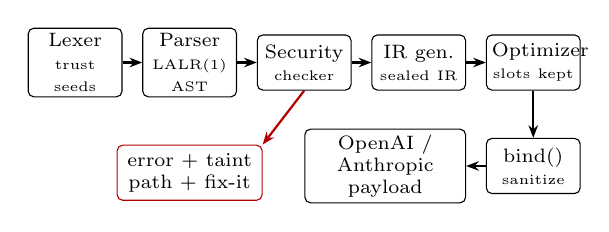
\begin{tikzpicture}[
  node distance=3mm and 2.5mm,
  box/.style={draw, rounded corners=2pt, align=center, font=\scriptsize, minimum height=7mm, inner sep=2pt, text width=10.5mm},
  arr/.style={-{Stealth[length=1.6mm]}, thick}]
\node[box] (lex) {Lexer\\\tiny trust seeds};
\node[box, right=of lex] (par) {Parser\\\tiny LALR(1) AST};
\node[box, right=of par] (sem) {Security\\\tiny checker};
\node[box, right=of sem] (gen) {IR gen.\\\tiny sealed IR};
\node[box, right=of gen] (opt) {Optimizer\\\tiny slots kept};
\node[box, below=6mm of opt] (bind) {bind()\\\tiny sanitize};
\node[box, left=of bind, text width=19mm] (pay) {OpenAI /\\Anthropic payload};
\node[box, below=6mm of par, text width=17mm, draw=red!70!black] (err) {error + taint\\path + fix-it};
\draw[arr] (lex) -- (par);
\draw[arr] (par) -- (sem);
\draw[arr] (sem) -- (gen);
\draw[arr] (gen) -- (opt);
\draw[arr] (opt) -- (bind);
\draw[arr] (bind) -- (pay);
\draw[arr, red!70!black] (sem.south) -- (err.north east);
\end{tikzpicture}
\caption{Compiler pipeline. All phases above run at compile time; only \code{bind()} runs per request.}
\label{fig:pipeline}
\end{figure}

\textbf{Lexical analysis.} A PLY tokenizer records exact spans and seeds each token's intrinsic trust (literals \lab{TRUSTED}, names after \code{input} by source). Strings are split during lexing into text and \code{\{hole\}} parts, so later phases can point at the exact leaking hole. \textbf{Syntax analysis.} An LALR(1) grammar with error productions gives targeted hints (e.g.\ a bare variable in a block suggests \code{insert(x)}). Because LALR state merging over-reports acceptable tokens, the parser computes exact ``expected'' sets by simulating pending reductions per candidate token. \textbf{Semantic analysis.} Name resolution with close-match hints, the trust lattice, symbolic evaluation, pattern analysis, taint paths reported as secondary source locations, and machine-applicable fix-its that are re-checked before being offered:
\begin{lstlisting}[language={},basicstyle=\ttfamily\scriptsize]
error[TL-S010]: UNTRUSTED data from input `user_msg`
                reaches a `system` block
 --> prompt.tlx:5:12
5 |     insert(user_msg)
  |            ^~~~~~~~ raw input inserted here
  = help: insert(sanitize(user_msg))
\end{lstlisting}
\textbf{Intermediate code.} The IR keeps text parts and input slots separate, is canonical JSON with a SHA-256 checksum, and can carry an HMAC-SHA256 seal; \code{generate()} re-verifies its own output. \textbf{Optimization.} Rule-based rewriting of developer text to a fixpoint, with correctness defined as whitespace equivalence with the slot sequence preserved and property-tested (idempotent, never grows, keeps the invariant); at \code{-O1} the example shrinks by 8--13\%. \textbf{Binding.} A registry of named sanitizers; the default performs NFKC normalization, removes control, zero-width and bidi characters, defuses chat-template role markers, caps length, and \emph{spotlights}~\cite{hines2024spotlighting} the value in \code{<untrusted\_input>} delimiters it cannot close early.

% =====================================================================
\section{Complexity Analysis}\label{sec:complexity}

Let $n$ be the program size, $S$ the largest template built, and $m$ the IR size. Lexing and LALR(1) parsing are $O(n)$; name resolution is $O(n)$ expected; the security analysis is $O(n\cdot S)$, since each statement copies at most $S$ template parts and joins are over a constant-height lattice; pattern analysis is linear in the pattern; IR generation, checksumming and sealing are $O(m)$; the optimizer is $O(k\cdot m)$ for $k$ fixpoint rounds, with $k\le m$ because every rewrite except one-time normalization strictly shortens the text; binding is linear in $m$ plus the input length. No flow analysis runs per request.

\textbf{Typical programs.} When no value is repeatedly duplicated, $S$ is bounded by the program text and scaling is near-linear. Measured on an AMD Ryzen laptop (Python 3.10, median of 5 runs), compile time grows from 4.7\,ms for 10 statements to 44\,ms for 100, 207\,ms for 500 and 3.77\,s for 5{,}000, i.e.\ 0.41--0.75\,ms per statement (log--log slope 1.14 for $n\ge100$); lexing and parsing take 63--80\% of the time. The example program compiles in about 5\,ms.

\textbf{Worst case.} Because templates are copied, $k$ repetitions of \code{a = a + a} build $2^k$ parts: compile time is 18.8\,ms at $k{=}10$, 305\,ms at $k{=}14$ and 2.69\,s at $k{=}17$, doubling with each statement. The cost is proportional to the prompt being built---inserting the value yields $2^{17}$ slots, beyond any model's context window---and can be bounded independently of output size by hash-consing templates into a DAG or by a size cap tied to the largest context window. The blow-up is not reachable by an attacker: the program is written by the trusted developer, and attacker-controlled values enter only at bind time, whose cost is linear in their length.

% =====================================================================
\section{Evaluation}\label{sec:eval}

\subsection{Setup}
\textbf{Corpus:} 48 hand-written programs (26 unsafe, 22 safe) in 14 categories, 32 attacks in 8 categories (direct override, role tokens, nested role tokens, transcript forgery, delimiter escape, Unicode obfuscation, payload splitting, social engineering), and 10 benign inputs. \textbf{Baselines:} B1, a lexical linter; B2, a keyword blocklist on the naively rendered prompt; and a naive string-concatenation renderer. \textbf{Live models} (free API tiers, temperature 0, at most 1{,}024 output tokens): \code{openai/gpt-oss-20b} and \code{allam-2-7b} (Groq) and \code{gemma-4-26b-a4b-it} (Google). \textbf{Public benchmark:} from the Tensor Trust hijacking set~\cite{toyer2024tensortrust} (776 human-written attacks) we keep the 206 distinct attacks that name the target phrase ``Access Granted'' within 800 characters, replace the phrase with our canary, and sample 64 with a fixed seed. \textbf{Judging:} each trial embeds a fresh random canary; an attack succeeds if the reply contains it in a sentence that is not a refusal. \textbf{Statistics:} Wilson 95\% intervals~\cite{wilson1927} and exact McNemar tests~\cite{mcnemar1947} on paired trials.

\subsection{Detection and structural leakage}
Table~\ref{tab:detect} compares detection. A perfect score for \TL{} is expected, since its analysis is exact for the language and the corpus was written by the authors; the evidence beyond this corpus is the property-based test of Theorem~\ref{thm:ni} on random programs. The corpus shows where lightweight alternatives fail. B1 misses every leak through variables or reassignment; B2 catches all leaks only because it sees the naive rendering, and flags 13 of 22 safe programs.

\begin{table}[t]
\caption{Detection on the labelled corpus (unsafe = positive)}
\label{tab:detect}
\centering
\resizebox{\columnwidth}{!}{%
\begin{tabular}{@{}lrrrrccc@{}}
\toprule
Method & TP & FP & FN & TN & Prec. & Rec. & F1 \\
\midrule
\TL{} & 26 & 0 & 0 & 22 & \textbf{1.00} & \textbf{1.00} & \textbf{1.00} \\
B1 lexical & 13 & 8 & 13 & 14 & 0.62 & 0.50 & 0.55 \\
B2 keyword & 26 & 13 & 0 & 9 & 0.67 & 1.00 & 0.80 \\
\bottomrule
\end{tabular}}
\end{table}

Across all 1{,}536 program--attack pairs, a \emph{structural leak}---a role token, a forged transcript turn or a delimiter break-out reaching the system message---occurs in 38.1\% of pairs under naive rendering and in 0\% under \TL{} (832 pairs blocked at compile time, 96 at bind time, 608 rendered with no surviving structure). B2 catches only 56.2\% of the naive pairs in which an attack reaches the system message while flagging 30\% of benign inputs.

\subsection{Live attack success}
\textbf{Conditions.} Direct: \textbf{A} customer message raw in the system prompt; \textbf{B} raw in the user turn; \textbf{C} the \TL{} program (sanitized and spotlighted in the user turn); \textbf{D} C plus typed fields that the attacker also writes. Indirect (RAG): the question is harmless and the attacker controls a retrieved article; \textbf{A} article raw in the system prompt (rejected by \TL{} with \code{TL-S011}); \textbf{B} raw in the user turn; \textbf{C} \TL{}. A free-text article admits no refinement type, so there is no D. Table~\ref{tab:asr} gives the results.

\begin{table}[t]
\caption{Attack success rate (\%) by condition. Ours = our 32 attacks (2 repeats where $n{=}64$); TT = 64 Tensor Trust attacks; Dir./Ind. = direct/indirect scenario; $n$ = attack trials per condition. D blocks before any request.}
\label{tab:asr}
\centering
\resizebox{\columnwidth}{!}{%
\begin{tabular}{@{}llrrrrr@{}}
\toprule
Model & Attacks & $n$ & A & B & C & D \\
\midrule
\multirow{4}{*}{gpt-oss-20b} & Ours, Dir. & 32 & 25.0 & 12.5 & 9.4 & \textbf{0} \\
 & Ours, Ind. & 32 & 28.1 & 18.8 & \textbf{6.2} & -- \\
 & TT, Dir. & 64 & 23.4 & 18.8 & 18.8 & \textbf{0} \\
 & TT, Ind. & 32 & 43.8 & 25.0 & 31.2 & -- \\
\midrule
\multirow{4}{*}{allam-2-7b} & Ours, Dir. & 64 & 48.4 & 42.2 & 48.4 & \textbf{0} \\
 & Ours, Ind. & 64 & 57.8 & 59.4 & \textbf{40.6} & -- \\
 & TT, Dir. & 64 & 62.5 & 70.3 & 59.4 & \textbf{0} \\
 & TT, Ind. & 64 & 75.0 & 73.0 & \textbf{56.2} & -- \\
\midrule
\multirow{4}{*}{gemma-4-26b} & Ours, Dir. & 64 & 4.7 & 1.6 & 0.0 & \textbf{0} \\
 & Ours, Ind. & 64 & 6.2 & 0.0 & 0.0 & -- \\
 & TT, Dir. & 64 & 1.6 & 1.6 & 1.6 & \textbf{0} \\
 & TT, Ind. & 64 & 4.7 & 1.6 & 1.6 & -- \\
\bottomrule
\end{tabular}}
\end{table}

\textbf{Findings.} (1)~\emph{Typed inputs block every attack on every model before any API call.} D's 0\% holds by construction: it shows that a refinement-typed field cannot carry an injection, independent of the model. (2)~\emph{The public attacks are stronger}: on allam-2-7b they succeed in 56--75\% of trials versus 41--59\% for ours, yet D still blocks all of them. (3)~\emph{\TL{}'s layout significantly reduces indirect injection.} With the attack in a retrieved document, C is significantly lower than both naive layouts on allam-2-7b for both attack sets (exact McNemar, A vs.\ C $p=0.043$ and $0.017$; B vs.\ C $p=0.029$ and $0.013$), and lower than the system-prompt layout on gpt-oss-20b with our attacks (28.1\% to 6.2\%, $p=0.016$). With Tensor Trust attacks on gpt-oss-20b, C (31.2\%) is below A (43.8\%) but not significantly, and not below B. In the direct scenario no difference between A, B and C is significant: spotlighting marks data, but the customer's own message is addressed to the model anyway. (4)~\emph{Spotlighting needs a model that respects delimiters.} allam-2-7b, a 7B model without instruction-hierarchy training, often repeats codes found anywhere in its context, so only the compile-time guarantees fully protect it; this agrees with findings that prompt-level defences depend on model training~\cite{hines2024spotlighting,chen2025struq}. (5)~\emph{A strongly aligned model} (gemma-4) resists all conditions, so they cannot be separated. Utility on benign inputs stayed between 80\% and 100\% in every condition, and \TL{} conditions were never more than one request below the naive ones.

\subsection{Comparison with existing work}\label{sec:compare}
Table~\ref{tab:compare} sets our measured values beside the alternatives we implemented and the results that existing defences report. The published figures come from different models, attack sets and threat models, so they are context rather than a head-to-head ranking; the qualitative comparison is in Table~\ref{tab:related}.

\begin{table}[t]
\caption{Measured and reported results of prompt-injection defences}
\label{tab:compare}
\centering
\resizebox{\columnwidth}{!}{%
\begin{tabular}{@{}p{2.3cm}p{1.9cm}p{4.4cm}@{}}
\toprule
Approach & Acts at & Result (source) \\
\midrule
B1 lexical linter & dev.\ time & F1 0.55; misses 13 of 26 unsafe programs (ours) \\
B2 keyword filter & run time & catches 56.2\% of attacks reaching the system prompt; flags 30\% of benign inputs (ours) \\
Spotlighting~\cite{hines2024spotlighting} & prompt & ASR from $>$50\% to $<$2\% on GPT-family models (reported) \\
StruQ~\cite{chen2025struq} & model training & significantly better resistance, little or no utility loss (reported, qualitative) \\
CaMeL~\cite{debenedetti2025camel} & run time & 77\% of AgentDojo tasks solved with provable security vs.\ 84\% undefended (reported) \\
\midrule
\textbf{\TL{}} & compile time & F1 1.00; structural leaks 38.1\%$\to$0\%; typed inputs 100\% blocked; indirect ASR vs.\ user-turn placement 73.0$\to$56.2\% (allam, $p{=}0.013$), vs.\ system placement 28.1$\to$6.2\% (gpt-oss, $p{=}0.016$); utility 80--100\%; $\approx$5\,ms compile, no per-request model call (ours) \\
\bottomrule
\end{tabular}}
\end{table}

Three points stand out. First, unlike the keyword filter, \TL{} decides from where text is placed rather than what it says, so it has no false positives on benign inputs and its compile-time verdict cannot be evaded by rephrasing an attack. Second, our spotlighting gains are smaller than the figure Hines et al.\ report; their experiments use GPT-family models and their own spotlighting variants and attacks, while we use the default delimiting sanitizer with smaller open models and include the public Tensor Trust attacks, so the comparison illustrates how strongly prompt-level defences depend on the model and the attacks. This is exactly why \TL{} pairs spotlighting with model-independent compile-time guarantees. Third, CaMeL and StruQ protect a different layer (agent tool calls and model weights) and compose with \TL{}: a \TL{} program can supply the trusted prompt of a CaMeL-style system or be sent to a StruQ-trained model.

\subsection{Guidance for developers}
The results suggest a layered use of \TL{}. (1)~Give every input whose values can be enumerated or bounded a refinement type: such inputs blocked every attack on every model before any request. (2)~Keep customer messages and retrieved documents in the \code{instruction} channel, sanitized and spotlighted; this layout significantly reduced indirect injection on two of the three models. (3)~Treat \code{sanitize()} inside \code{system} as a reviewed declassification, reserved for short values such as a customer's name. (4)~Send the compiled prompt to a model trained to respect the instruction hierarchy~\cite{wallace2024hierarchy}, since the remaining risk lies in persuasion within the user turn, which no prompt-construction discipline can remove.

% =====================================================================
\section{Limitations and Threats to Validity}

The guarantee covers the privileged channel: untrusted text is still allowed, delimited, in the user turn, where a model can still be persuaded. \code{sanitize()} is only as strong as the sanitizer, which removes structural vectors but cannot neutralize natural-language instructions in general. Validation is syntactic: a permissive pattern such as \code{[A-Za-z]\{1,40\}} admits a single word. Completeness relies on straight-line programs; with branches the analysis would stay sound but not complete. The worst case is exponential (Section~\ref{sec:complexity}). Our corpus and attacks are hand-written, which the Tensor Trust benchmark mitigates; that benchmark was written against the game's defences rather than our application, and attacks that spell the target phrase indirectly are excluded. We test three free-tier models with 32--64 attacks per condition (32 for gpt-oss-20b on indirect Tensor Trust attacks, owing to the provider's daily token quota), so intervals are wide; repeats at temperature 0 vary only the canary. Canary-based success is a proxy; a refusal-aware judge avoids counting refusals that quote the canary, and empty replies (gpt-oss reasoning that exhausted the output budget, or a provider's safety filter) count as unsuccessful attacks; they occur mostly in the naive condition~A, and excluding them moves no success rate by more than 4.5 points and changes no significance verdict. The fix-it for \code{TL-S010} proposes the minimal type-correct change, sanitizing in place; moving the value to the \code{instruction} channel is usually preferable, and a policy that forbids declassification into \code{system} is future work.

% =====================================================================
\section{Conclusion}

Prompt injection in LLM-integrated applications is in part a construction problem: trusted instructions and untrusted data are concatenated into one string. \TL{} borrows the remedy that programming languages applied to SQL injection and cross-site scripting, making the trust of every piece of text part of the program's type and refusing to build an unsafe prompt, while acknowledging that, unlike a database engine, a model can still be persuaded by data it is shown. Its exact analysis yields non-interference for the privileged channel with no false positives, and its compiled output carries the guarantee to the API call. The experiments show the layers working together: refinement types block attacks independently of the model, channel separation keeps untrusted text out of the system prompt, and spotlighting adds a model-dependent reduction that is significant only for indirect injection. Future work includes DAG-shared templates, control flow with sound joins, trust tracking across multi-step agent pipelines, integration with capability-based runtimes, and a language server for live diagnostics.

\section*{Acknowledgment}

The authors thank Dr.~Krishnaraj~N for his guidance throughout this work.

\textbf{Use of AI tools.} In accordance with IEEE policy on AI-generated content, the authors disclose that Claude (Anthropic), used through the Claude Code assistant, served as an assistant in this work: for debugging and extending the compiler and its automated test suite, for building and running the evaluation harness and its statistical analysis, and for drafting the manuscript text and its \LaTeX{} layout. The concept and design of \TL{}, the direction of the work and all final decisions are the authors'; the authors reviewed and tested all code, verified every reported number against the logged results, and take full responsibility for the content of this paper. The language models evaluated in this paper are subjects of the experiments, not authoring tools (Section~\ref{sec:eval}).

\bibliographystyle{IEEEtran}
\bibliography{refs}

\end{document}
